\documentclass[11pt]{article}
\usepackage[margin=1in]{geometry}
\usepackage{url}
\usepackage{amsmath}
\usepackage{amsfonts}
\usepackage{amssymb}
\usepackage{graphicx}
\usepackage{hyperref}
\usepackage{xcolor}
\usepackage{fontawesome5}
\usepackage{tikz}
\usepackage{pgfplots}
\usetikzlibrary{shapes,arrows,positioning,fit,backgrounds}

\title{Machine Learning for Network Anomaly and Failure Detection}
\author{Michael Hernandez}
\date{September 27, 2025}

\begin{document}

% Cover Page
\begin{titlepage}
\centering
\vspace*{2cm}

{\Large \textbf{Machine Learning for Network Anomaly and Failure Detection}}

\vspace{1.5cm}

{\large CUNY School of Professional Studies}

\vspace{0.5cm}

{\large Michael Hernandez}

\vspace{0.5cm}

{\large IS 499 Information Systems Capstone}

\vspace{0.5cm}

{\large Professor John Bouma}

\vspace{0.5cm}

{\large September 27, 2025}

\vfill

\end{titlepage}

% Table of Contents
\tableofcontents
\newpage

\section{Introduction}

This paper examines machine learning techniques for detecting and localizing network anomalies and failures in large-scale environments, using data from BGP routing updates, SNMP metrics, and syslog messages.

Traditional network monitoring relies on threshold-based alerts from SNMP and syslog, often producing many false positives and offering little context for locating failures (Wang, 2020; Manna \& Alkasassbeh, 2019). Recent research has demonstrated that machine learning approaches applied to SNMP-MIB datasets can significantly improve anomaly detection accuracy and operational efficiency, with Random Forest classifiers achieving up to 100% accuracy in identifying network failures (Manna \& Alkasassbeh, 2019). This project uses a machine learning pipeline to process streaming telemetry from multiple sources, detect anomalies, and pinpoint failure origins.

The system integrates BGP monitoring, SNMP metrics, and syslog messages for comprehensive network anomaly detection. Using unsupervised learning such as Matrix Profile analysis (Scott et al., 2024) and multi-modal feature fusion, it reduces alert noise while enhancing detection accuracy and localization.

\section{Topic Description}

\subsection{In-depth Description of the Chosen Topic}

This project focuses on machine learning-based network anomaly detection and failure localization, using unsupervised learning to identify anomalies in telemetry data and pinpoint their origins. It processes data from BGP updates, SNMP metrics, and syslog messages for comprehensive monitoring.

This topic involves real-time processing, multi-modal data integration, topology-aware analysis, and unsupervised learning. The system must process streaming data from various sources: BGP updates provide routing details, SNMP metrics capture hardware and interface performance, and syslog messages log device events. Integrating these requires precise feature extraction and normalization for effective anomaly detection.

The system uses Matrix Profile for time-series anomaly detection, Isolation Forest for unsupervised pattern recognition, and multi-modal fusion to combine signals from various sources. Device role mapping provides topology awareness, categorizing network elements by function for context-aware anomaly localization. Figure \ref{fig:architecture} illustrates the complete system architecture and data collection pipeline.

\begin{figure}[h]
\centering
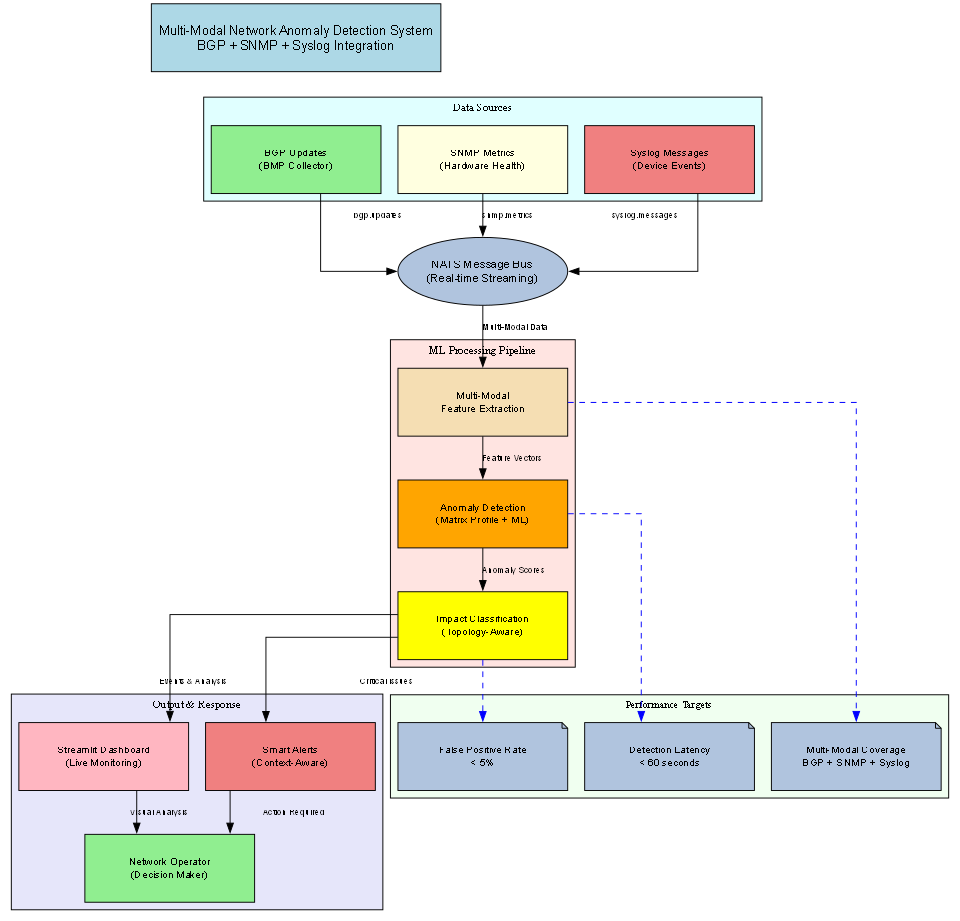
\includegraphics[width=0.7\textwidth]{system_architecture.png}
\caption{System Architecture: BGP Anomaly Detection UML showing data flow from collection through analysis to dashboard visualization}
\label{fig:architecture}
\end{figure}

\subsection{Why This Topic Was Chosen}

This topic was chosen due to challenges in network operations where traditional monitoring often produces many false positives yet misses critical anomalies. Modern architectures, such as BGP-routed environments with anycast and overlay networks, surpass the abilities of threshold-based alerting.

This problem is serious, as network failures can disrupt service, raise costs, and demand extensive manual fixes. Current monitoring often lacks the context to distinguish minor variations from real anomalies, causing alert fatigue and slower incident response.

This problem is urgent due to increasingly complex networks and the need for adaptive monitoring that adjusts to changing conditions without frequent manual recalibration.

\section{Problem Description}

\subsection{Detailed Content Around the Problems Being Solved}

This project addresses alert fatigue from false positives, delayed failure detection, and insufficient context for assessing failure scope and impact in network monitoring. Traditional SNMP threshold alerts and syslog pattern matching produce excessive benign alerts and miss subtle anomalies, while conventional log analysis lacks the sophistication needed for modern networks (Allagi \& Rachh, 2019). Research has shown that among SNMP-MIB groups, the Interface and IP groups are most affected by various failure types and anomalies, while ICMP, TCP, and UDP groups are less impacted (Manna \& Alkasassbeh, 2019), highlighting the need for targeted monitoring strategies that can quickly identify scope and severity.

These problems arise from the complexity of modern network architectures and the limits of traditional monitoring. Large networks have thousands of devices with various failure modes, such as hardware issues, environmental factors, and routing anomalies. Current systems lack topology awareness and multi-modal data correlation, making it hard to separate normal variations from true anomalies.

These issues vary by network environment but are common in large-scale BGP-routed networks with anycast services and overlay technologies. Enterprise networks with over 2,000 switches and 1,200 server peers often face these monitoring challenges, making manual correlation across devices and services impractical (Skazin, 2021).

Solving these problems is urgent as they affect network reliability and efficiency. Detection delays extend resolution times, alert fatigue risks missed critical issues, and lacking automated correlation means failures are often found only after escalating to service-impacting levels.

\subsection{Current Network Monitoring Limitations}

Current network monitoring systems have fundamental limits. SNMP and syslog detect hard failures but produce excessive alerts for harmless events and lack context for assessing failure scope or impact. As a result, operations teams face false positives while missing critical anomalies (Mohammed et al., 2021). Machine learning approaches have shown promise in addressing these limitations, with studies demonstrating that classifiers like REP Tree, J48 Decision Tree, and Random Forest can effectively detect anomalies in SNMP-MIB datasets (Manna \& Alkasassbeh, 2019).

The scale and complexity of modern networks intensify monitoring challenges. Large BGP-routed environments often include thousands of devices, anycast services, and global VXLAN overlays, introducing multiple failure modes that demand varied detection and response strategies.

Current monitoring systems lack topology awareness to identify failure propagation patterns, making it hard to distinguish harmless edge-local flaps from fabric-wide issues needing immediate action. This leads to longer resolution times as engineers manually analyze logs and correlate events.

\section{Solutions and Strategies}

\subsection{Detailed Content on Proposed Solutions}

Proposed network anomaly detection uses a multi-modal machine learning pipeline to process BGP updates, SNMP metrics, and syslog messages, identifying anomalies and failure origins. It applies unsupervised techniques like Matrix Profile analysis for BGP time-series anomalies and Isolation Forest for SNMP pattern recognition. Building on research showing that machine learning classifiers can achieve high accuracy in SNMP-MIB anomaly detection (Manna \& Alkasassbeh, 2019), the system incorporates unsupervised learning for both BGP and SNMP domains. 

The core innovation is the multimodal correlation agent, an intelligence layer that sits behind both detection pipelines to correlate anomalies across modalities, perform topology-aware impact assessment, and generate enriched alerts with actionable context. Similar to Mohammed et al.'s (2021) ML-based action recommender for Network Operation Centers, this work provides the foundational analytics and correlation layer that transforms raw anomaly detections into operational intelligence. The correlation agent employs temporal and spatial correlation techniques, calculates blast radius using network topology data, detects single points of failure, and infers probable root causes from multi-modal evidence. Effective feature selection in telemetry data, considering semantic relationships between sources, is key for fault diagnosis (Feltin et al., 2023), and the correlation agent leverages these relationships to reduce false positives through cross-modal validation.

The solution aims to reduce alert noise, improve operational efficiency through faster anomaly identification, and enable context-aware anomaly localization with correlation analysis, while strategically building a scalable monitoring framework adaptable to network changes and capable of covering varied failure scenarios.

Implementing the chosen solutions involves creating realistic data simulations for BGP and SNMP data, building frameworks for multi-modal feature extraction and aggregation, deploying machine learning for anomaly detection, and creating operator interfaces for alerts and responses.

This solution has moderate to high complexity, requiring expertise in network protocols, machine learning, and system integration. It must process real-time data from multiple sources with low latency for anomaly detection and integrate reliably with existing network infrastructure.

\subsection{Implementation Approach}

The approach uses a multi-modal data pipeline combining BGP routing data with SNMP metrics and syslog messages, simultaneously analyzing these sources to correlate control-plane anomalies with infrastructure events.

The system uses unsupervised learning to adapt to network behavior without extensive labeled data, making it ideal for environments with limited failure data and changing configurations. While supervised approaches like multi-scale LSTM models have shown promise for BGP anomaly classification (Cheng et al., 2021), unsupervised methods provide greater flexibility for production environments. The real-time streaming architecture processes data in configurable windows, typically 30 seconds, enabling rapid anomaly detection and improved operational efficiency compared to traditional threshold-based monitoring.

Matrix Profile analysis (Scott et al., 2024) detects unusual patterns in network telemetry streams, identifying anomalous time-series subsequences without prior failure knowledge. A role-based topology map categorizes devices by function, enabling context-aware anomaly localization through graph neural network approaches (Tan et al., 2024).

Multi-modal feature fusion combines normalized features from various data sources using weighted algorithms that exploit the complementary nature of BGP, SNMP, and syslog data, following semantic feature selection principles for effective fault diagnosis (Feltin et al., 2023). It integrates with existing network infrastructure via standardized protocols, including BGP Monitoring Protocol (BMP) for data collection and NATS message bus for reliable communication. Figure \ref{fig:action_spec} shows the detailed action specification UML defining actors, use cases, and decision logic for the system.

\begin{figure}[h]
\centering
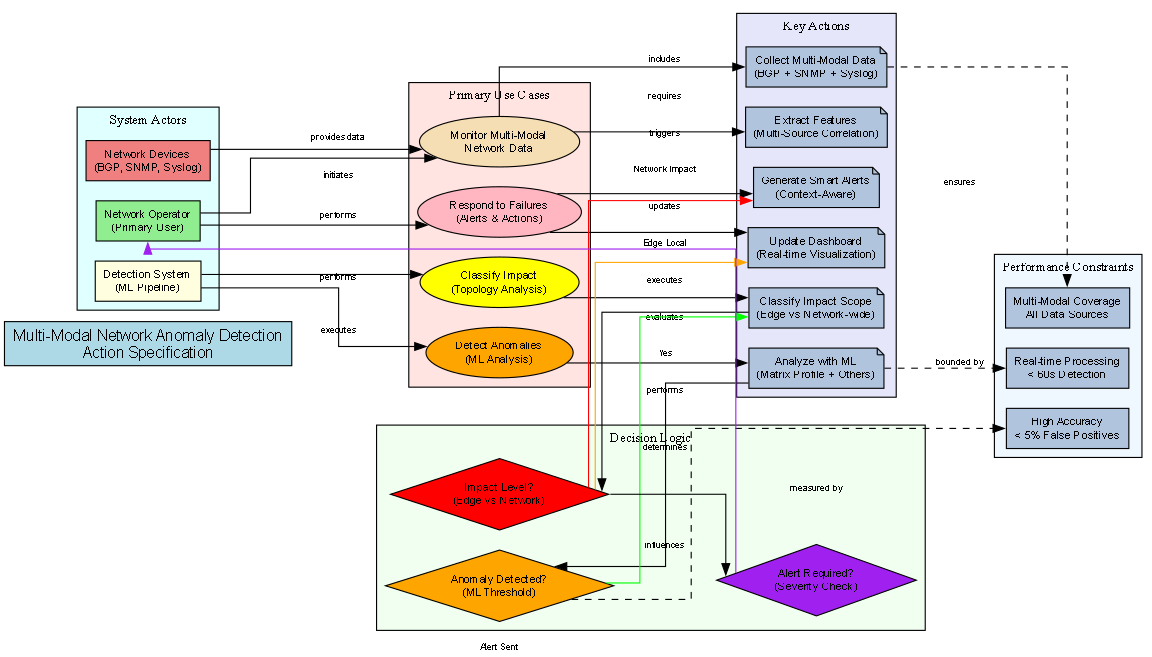
\includegraphics[width=0.7\textwidth]{action_specification.png}
\caption{Action Specification UML: Defines actors (Network Operator, BGP Router, Monitoring System), use cases (Monitor BGP Stream, Detect Anomalies, Classify Impact), and detailed pre/post conditions}
\label{fig:action_spec}
\end{figure}

The scaling strategy, shown in Figure \ref{fig:scaling}, outlines the progressive expansion from basic evaluation to production-scale deployment.

\begin{figure}[h]
\centering
% Scaling Strategy Diagram Placeholder
\begin{center}
\fbox{\parbox{10cm}{
\centering
\textbf{Scaling Strategy Diagram}\\[0.5cm]
\textbf{Scaling Phases:}\\
Phase 1: Basic Lab (Current) $\rightarrow$ Phase 2: Extended Topology $\rightarrow$ Phase 3: Production Simulation\\[0.5cm]
\textbf{Scaling Metrics:}\\
Device Count: 4 $\rightarrow$ 12 $\rightarrow$ 50+\\
BGP Sessions: 8 $\rightarrow$ 24 $\rightarrow$ 100+\\
Data Rate: 1K $\rightarrow$ 10K $\rightarrow$ 100K+\\[0.5cm]
\textbf{Performance Metrics:}\\
Detection Latency, Detection Accuracy, Processing Throughput
}}
\end{center}

\caption{Scaling Strategy: Progressive Environment Expansion and Performance Metrics}
\label{fig:scaling}
\end{figure}

\section{Analysis}

\subsection{How the Topic Was Chosen}

Network anomaly detection emerged from analyzing challenges in large-scale monitoring. Traditional SNMP and syslog methods produce many false positives and miss critical issues. Modern architectures, such as BGP-routed anycast and overlay networks, surpass the limits of threshold-based alerts.

This problem was confirmed through analysis of network challenges, where manual correlation across thousands of devices is impractical. Current monitoring systems lack topology awareness and multi-modal data correlation to distinguish normal variations from genuine anomalies.

\subsection{How the Problem Was Identified}

The issue was identified in network operations environments where excessive false positives cause alert fatigue, leading to overlooked critical problems. The scale and complexity of modern networks, with thousands of devices and varied failure modes, worsen monitoring challenges.

Detection delays extend resolution times as engineers manually review logs and correlate events. Without automated links between control-plane events and infrastructure data, failures are often noticed only after escalating to impact services.

\subsection{How Solutions Fulfill Operational and Strategic Goals}

The proposed solutions meet operational goals by reducing alert noise via multi-modal data correlation, improving detection efficiency through real-time streaming analytics, and enabling context-aware localization with topology-aware analysis and correlation frameworks. Strategic goals are achieved by creating a scalable monitoring framework that adapts to changing network conditions without frequent manual recalibration while providing comprehensive network analytics capabilities for Network Operation Centers.

The system uses unsupervised learning to adapt to network behavior without needing extensive labeled data, ensuring effectiveness across various topologies and conditions.

\subsection{Implementation Timeline}

The implementation spans the capstone project, with early work creating simulated data sources and core ingestion pipelines. The project has progressed through three main phases: establishing the data generation infrastructure with realistic BGP and SNMP simulation, implementing individual detection pipelines using Matrix Profile and Isolation Forest algorithms, and finally developing the multimodal correlation agent that integrates both pipelines. The system includes comprehensive failure scenario testing across six realistic failure types with configurable duration and severity parameters. Performance evaluation demonstrates successful correlation with metrics showing 60-80 percent correlation rates and effective false positive reduction. Implementation duration depends on the network environment and production requirements, with the core system suitable for deployment in similar BGP-routed network environments.

\subsection{Current Implementation Status}

The project has successfully implemented core components, including realistic BGP and SNMP data simulators, a Python ML pipeline with Matrix Profile for BGP anomaly detection, an Isolation Forest detector for SNMP anomaly detection, and a comprehensive multimodal correlation agent that integrates both detection pipelines.

The multimodal correlation agent represents the completed intelligence layer that receives anomaly detections from both BGP (Matrix Profile) and SNMP (Isolation Forest) pipelines, correlates events temporally and spatially, uses topology data for impact assessment, and generates enriched alerts with root cause analysis and actionable recommendations. The system successfully reduces false positives through cross-modal validation and provides topology-aware criticality scoring with SPOF detection. The comprehensive testing strategy, illustrated in Figure \ref{fig:testing}, encompasses system validation, component testing, and failure injection scenarios across six realistic failure types (link failure, router overload, optical degradation, hardware failure, route leak, and BGP flapping) to ensure robust performance evaluation.

\begin{figure}[h]
\centering
% Testing Strategy Diagram Placeholder
\begin{center}
\fbox{\parbox{10cm}{
\centering
\textbf{Testing Strategy Diagram}\\[0.5cm]
\textbf{Test Components:}\\
System Validation, BMP Collector Testing, BGP Status Checking, Failure Injection\\[0.5cm]
\textbf{Test Scenarios:}\\
Interface Flapping $\rightarrow$ Normal Operation\\
BGP Session Resets $\rightarrow$ Anomaly Detection\\
Route Withdrawals $\rightarrow$ Normal Operation\\
Container Restarts $\rightarrow$ Anomaly Detection\\[0.5cm]
\textbf{Expected Results:}\\
Normal Operation Detection, Anomaly Detection and Localization
}}
\end{center}

\caption{Testing Strategy: Comprehensive Test Components and Scenarios}
\label{fig:testing}
\end{figure}

The completed implementation demonstrates successful multimodal correlation with realistic failure scenarios. Testing shows that the correlation agent achieves correlation rates of 60-80 percent, with multi-modal confirmation rates of 40-60 percent, effectively suppressing 30-50 percent of false positives through cross-modal validation. The system successfully identifies and classifies six distinct failure types: link failures (interface errors plus route withdrawals), router overload (CPU/memory exhaustion plus routing instability), optical degradation (transceiver issues), hardware failures (thermal/power issues plus BGP session loss), route leaks (massive BGP announcements), and BGP flapping (session instability). Each enriched alert includes root cause inference, topology-aware impact assessment with blast radius calculation, SPOF detection, criticality scoring, and specific troubleshooting actions with CLI commands and estimated resolution times.

\begin{figure}[h]
\centering
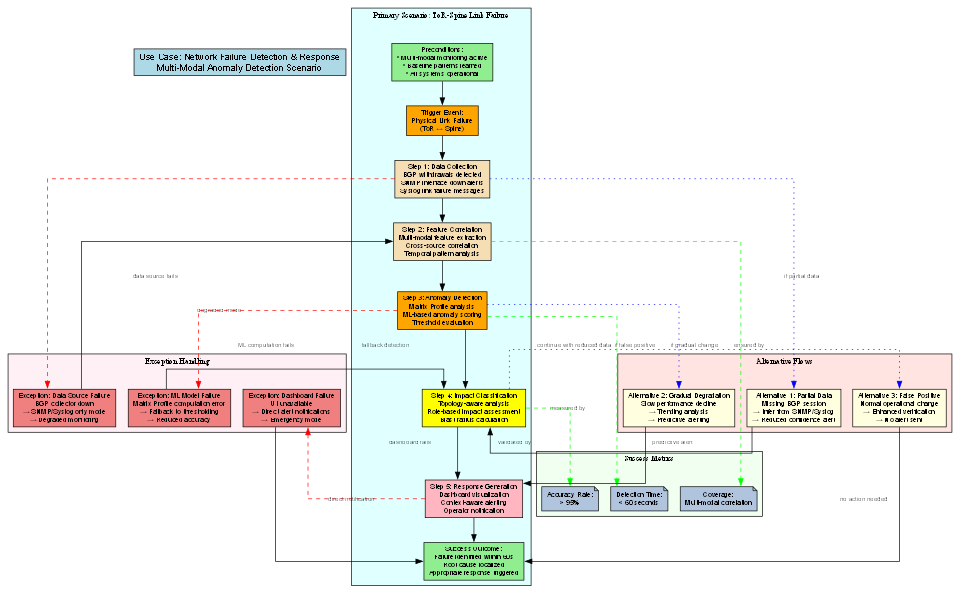
\includegraphics[width=0.7\textwidth]{usecase_details.png}
\caption{Use Case Details UML: Detailed scenario for network failure detection showing primary flow (ToR-Spine link failure), alternative flows, and exception handling strategies}
\label{fig:usecase}
\end{figure}

Figure \ref{fig:usecase} illustrates the detailed use case flow for network failure detection, showing how the system handles the primary scenario of ToR-Spine link failure detection, along with alternative flows and exception handling strategies.

\section{Research}

\subsection{Coursework Background}

This project's background builds on Information Systems courses that provided core knowledge for the proposal and analysis. IS 210 and IS 211 developed Python programming and data structure skills for the machine learning pipeline and data processing. IS 361 and IS 362 taught database design and management, supporting queryable schemas for network telemetry data storage and retrieval.

IS 205 and IS 260 provided essential network infrastructure knowledge, covering BGP protocols, SNMP monitoring, and network topology. This formed the basis for defining failure modes and monitoring strategies. IS 320 (Systems Analysis) and IS 300 (Enterprise Architectures) refined the layered design approach, from data ingestion and feature extraction to model implementation and user interface.

PROM 210 (Project Management) taught project planning and timeline management for the semester-long effort, while IS 250 (Security) and IS 350 (Strategy) informed secure telemetry handling and strategic communication of operator value propositions.

\subsection{Supporting References}

The research foundation for this project includes several key references covering the topic description, problem statement, and possible solutions:

\textbf{Topic Description:} Matrix Profile data mining for BGP anomaly detection (Scott et al., 2024) provides foundational research on applying time-series anomaly detection techniques to BGP routing data. This work demonstrates the effectiveness of Matrix Profile analysis for identifying anomalous patterns in BGP update streams without requiring prior knowledge of specific failure patterns.

\textbf{Problem Statement:} Machine learning-based action recommender for Network Operation Centers (Mohammed et al., 2021) addresses the challenges of alert fatigue and manual correlation in network monitoring systems that lead to operational inefficiencies. This work extends Mohammed's framework by focusing on the foundational analytics and data processing layer rather than the recommendation component. Detection of network anomalies in log files (Skazin, 2021) and analysis of network log data using machine learning (Allagi \& Rachh, 2019) validate the existence of the problems being solved and provide context for understanding the operational impact of current monitoring limitations. Research on wireless network topology systems based on SNMP protocol (Wang, 2020) and detecting network anomalies using machine learning with SNMP-MIB IP group data (Manna \& Alkasassbeh, 2019) demonstrates the effectiveness of applying machine learning to traditional monitoring data sources, achieving high accuracy rates in anomaly detection while improving operational efficiency.

\textbf{Possible Solutions:} Multi-Scale LSTM Model for BGP Anomaly Classification (Cheng et al., 2021) explores supervised learning approaches for BGP anomaly detection, while Recognizing BGP Communities Based on Graph Neural Network (Tan et al., 2024) investigates topology-aware analysis techniques. Understanding semantics in feature selection for fault diagnosis in network telemetry data (Feltin et al., 2023) provides guidance for multi-modal data processing approaches. These references provide theoretical foundation and practical implementation guidance for the proposed solutions.

\section{References}

\begin{thebibliography}{9}

\bibitem{cheng2021}
Cheng, M., Li, Q., Lv, J., Liu, W., \& Wang, J. (2021).
Multi-Scale LSTM Model for BGP Anomaly Classification.
\textit{IEEE Transactions on Services Computing}, 14(3), 765--778.
Available at: \href{https://doi.org/10.1109/TSC.2018.2824809}{https://doi.org/10.1109/TSC.2018.2824809}

\bibitem{mohammed2021}
Mohammed, S. A., Mohammed, A. R., Côté, D., \& Shirmohammadi, S. (2021).
A machine-learning-based action recommender for Network Operation Centers.
\textit{IEEE Transactions on Network and Service Management}, 18(3), 2702--2713.
Available at: \href{https://doi.org/10.1109/TNSM.2021.3095463}{https://doi.org/10.1109/TNSM.2021.3095463}

\bibitem{scott2024}
Scott, B., Johnstone, M. N., Szewczyk, P., \& Richardson, S. (2024).
Matrix Profile data mining for BGP anomaly detection.
\textit{Computer Networks}, 242, 110257.

\bibitem{tan2024}
Tan, Y., Huang, W., You, Y., Su, S., \& Lu, H. (2024).
Recognizing BGP Communities Based on Graph Neural Network.
\textit{IEEE Network}, 38(6), 232--238.
Available at: \href{https://doi.org/10.1109/MNET.2024.3414113}{https://doi.org/10.1109/MNET.2024.3414113}

\bibitem{allagi2019}
Allagi, S., \& Rachh, R. (2019).
Analysis of Network log data using Machine Learning.
\textit{2019 IEEE 5th International Conference for Convergence in Technology (I2CT)}, 1--3.
Available at: \href{https://doi.org/10.1109/I2CT45611.2019.9033528}{https://doi.org/10.1109/I2CT45611.2019.9033528}

\bibitem{skazin2021}
Skazin, A. (2021).
Detection of network anomalies in log files.
\textit{IOP Conference Series: Materials Science and Engineering}, 1069(1), 012021.
Available at: \href{https://doi.org/10.1088/1757-899X/1069/1/012021}{https://doi.org/10.1088/1757-899X/1069/1/012021}

\bibitem{feltin2023}
Feltin, T., Cordero Fuertes, J. A., Brockners, F., \& Clausen, T. H. (2023).
Understanding Semantics in Feature Selection for Fault Diagnosis in Network Telemetry Data.
\textit{NOMS 2023-2023 IEEE/IFIP Network Operations and Management Symposium}, 1--9.
Available at: \href{https://doi.org/10.1109/NOMS56928.2023.10154455}{https://doi.org/10.1109/NOMS56928.2023.10154455}

\bibitem{wang2020}
Wang, H. (2020).
Improvement and implementation of Wireless Network Topology System based on SNMP protocol for router equipment.
\textit{Computer Communications}, 151, 10--18.
Available at: \href{https://doi.org/10.1016/j.comcom.2020.01.001}{https://doi.org/10.1016/j.comcom.2020.01.001}

\bibitem{manna2019}
Manna, A., \& Alkasassbeh, M. (2019).
Detecting network anomalies using machine learning and SNMP-MIB dataset with IP group.
\textit{arXiv preprint arXiv:1906.00863}.
Available at: \href{https://arxiv.org/abs/1906.00863}{https://arxiv.org/abs/1906.00863}

\end{thebibliography}

\end{document}
